\documentclass[11pt]{article}
\usepackage[utf8]{inputenc}
\usepackage[english]{babel}
\usepackage[font=small,labelfont=bf]{caption}
\usepackage{geometry}
\usepackage{natbib}
\usepackage{hyperref}
\usepackage{pxfonts}
\usepackage{graphicx}
\usepackage{newfloat}
\usepackage{setspace}
%\doublespacing

\newcommand{\argmax}{\mathop{\mathrm{argmax}}\limits}

\title{\textit{Supplemental figures for}: A Gaussian process model of human electrocorticographic data}
\author{
  Lucy L. W. Owen$^{1}$,
  Tudor A. Muntianu$^{1}$,
  Andrew C. Heusser$^{1, 2}$, \\
  Patrick Daly$^{3}$,
  Katherine Scangos$^{3}$, and
  Jeremy R. Manning$^{1\ast}$\\\\
$^{1}$Department of Psychological and Brain Sciences, Dartmouth College,\\
Hanover, NH 03755, USA\\
$^{2}$Akili Interactive,\\
Boston, MA 02110, USA}

%\bibliographystyle{apa}

\begin{document}

\setcounter{equation}{0}
\setcounter{figure}{0}
\setcounter{table}{0}
\setcounter{page}{1}
\setcounter{section}{0}
\makeatletter
\renewcommand{\theequation}{S\arabic{equation}}
\renewcommand{\thefigure}{S\arabic{figure}}

\newcommand{\methods}{1}
\newcommand{\corrmaps}{2}
\newcommand{\freqs}{3}
\newcommand{\density}{4}
\newcommand{\infomap}{5}
\newcommand{\infomapfreqs}{6}

\begin{titlepage}
  \maketitle
\end{titlepage}

\begin{figure}[p]
\centering 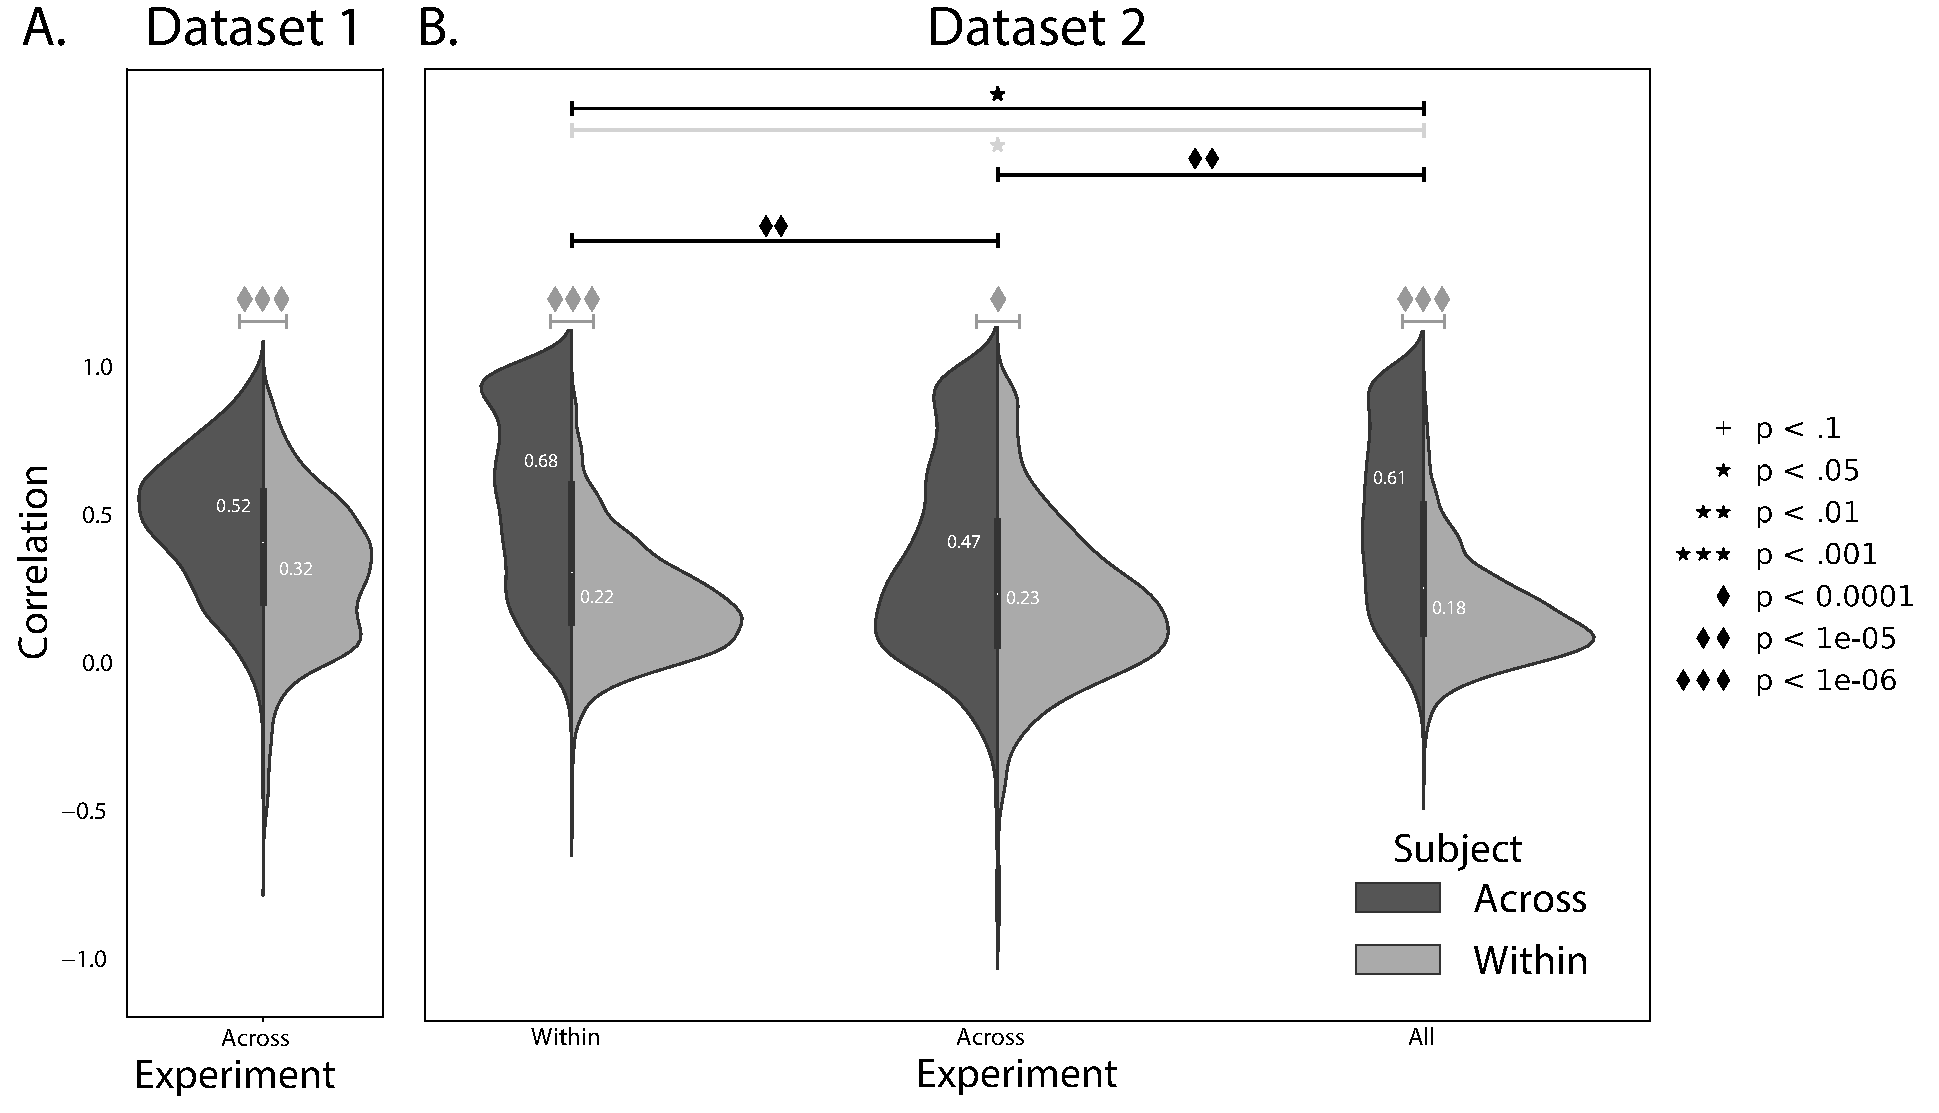
\includegraphics[width=\textwidth]{figs/supplemental_1}
\caption{\textbf{Reconstruction accuracy across all electrodes in two ECoG
datasets, broken down by experiment.} \textbf{A. Distributions of correlations
between observed versus reconstructed activity by electrode, for Dataset 1.}
The across-patient distribution (black) reflects reconstruction accuracy
(correlation) using a correlation model learned from all but one patient's data,
and then applied to that held-out patient's data. The within-patient
distribution (gray) reflects performance using a correlation model learned from
the same patient who contributed the to-be-reconstructed electrode.  The split
violin plot displays the same distributions shown in Figure~\corrmaps A.  The
white numbers within each half denote the means of each distribution. \textbf{B.
Distributions of correlations for Dataset 2.}  The split violin plots are in the
same format as those in Panel A.  The leftmost plot (``Within'') displays the
same distributions shown in Figure~\corrmaps B.  All reconstructions reflected
in the distribution were carried out using a model trained and tested using data
from the same experiment.  The middle plots (``Across'') reflect reconstructions
trained and tested using data from different experiments.  The rightmost plot
(``All'') reflect reconstructions obtained using models trained and tested on
data from both experiments.  The black distributions reflect models trained and
tested across patients (analogous to the black histograms in Figure~\corrmaps)
and the gray distributions reflect models trained and tested within patient
(analogous to the gray histograms in Figure~\corrmaps).  The dark gray
significance bars reflect paired-sample $t$-tests comparing the
($z$-transformed) reconstruction accuracy for each electrode obtained within
versus across patients.  The black significance bars reflect paired-sample
$t$-tests comparing the across-patient reconstruction accuracies across
datasets.  The light gray significance bars reflect paired-sample $t$-tests
comparing the within-patient reconstruction accuracies across datasets.  The
symbols denote the corresponding $p$-values of those statistical tests.}
\label{fig:supplemental_1}
\end{figure}


\begin{figure}[p]
\centering
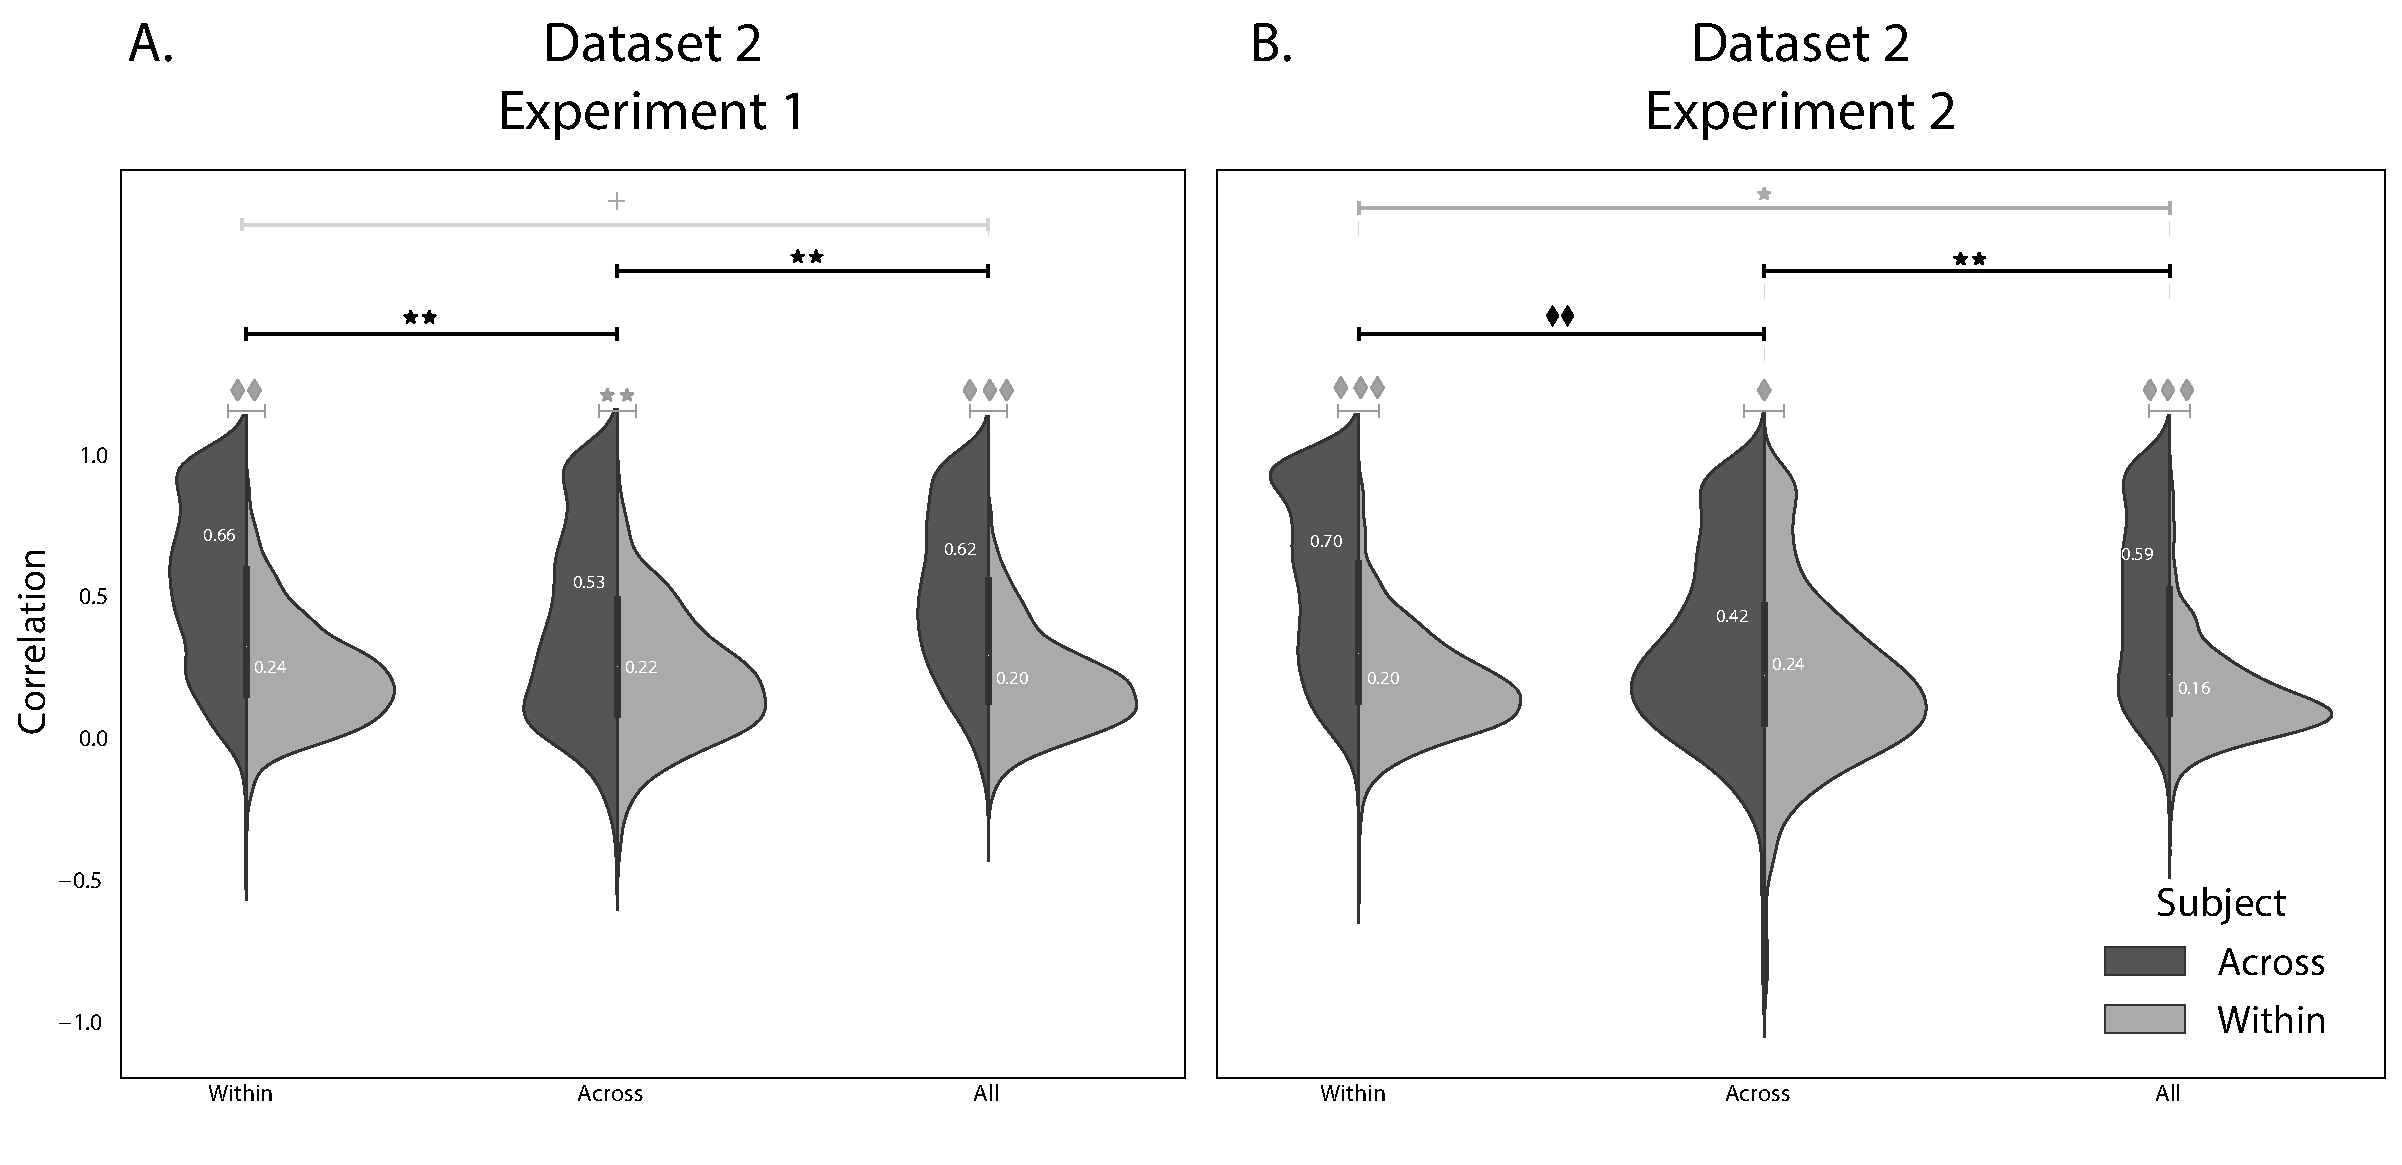
\includegraphics[width=\textwidth]{figs/supplemental_2}
\caption{\textbf{Reconstruction accuracy for Dataset 2, Experiments 1
    and 2.}  \textbf{A. Distributions of correlations between observed
    versus reconstructed activity by electrode, for Dataset 2
    (Experiment 1).}  The plots are in the same format as
  Figure~\ref{fig:supplemental_1}B, but reflect data only from
  Experiment 1 in Dataset 2.  \textbf{A. Distributions of correlations between observed
    versus reconstructed activity by electrode, for Dataset 2
    (Experiment 2).}  The plots are in the same format as Panel A, but
    reflect data only from Experiment 2 in Dataset 2.}
\label{fig:supplemental_2}
\end{figure}

\begin{figure}[p]
\centering 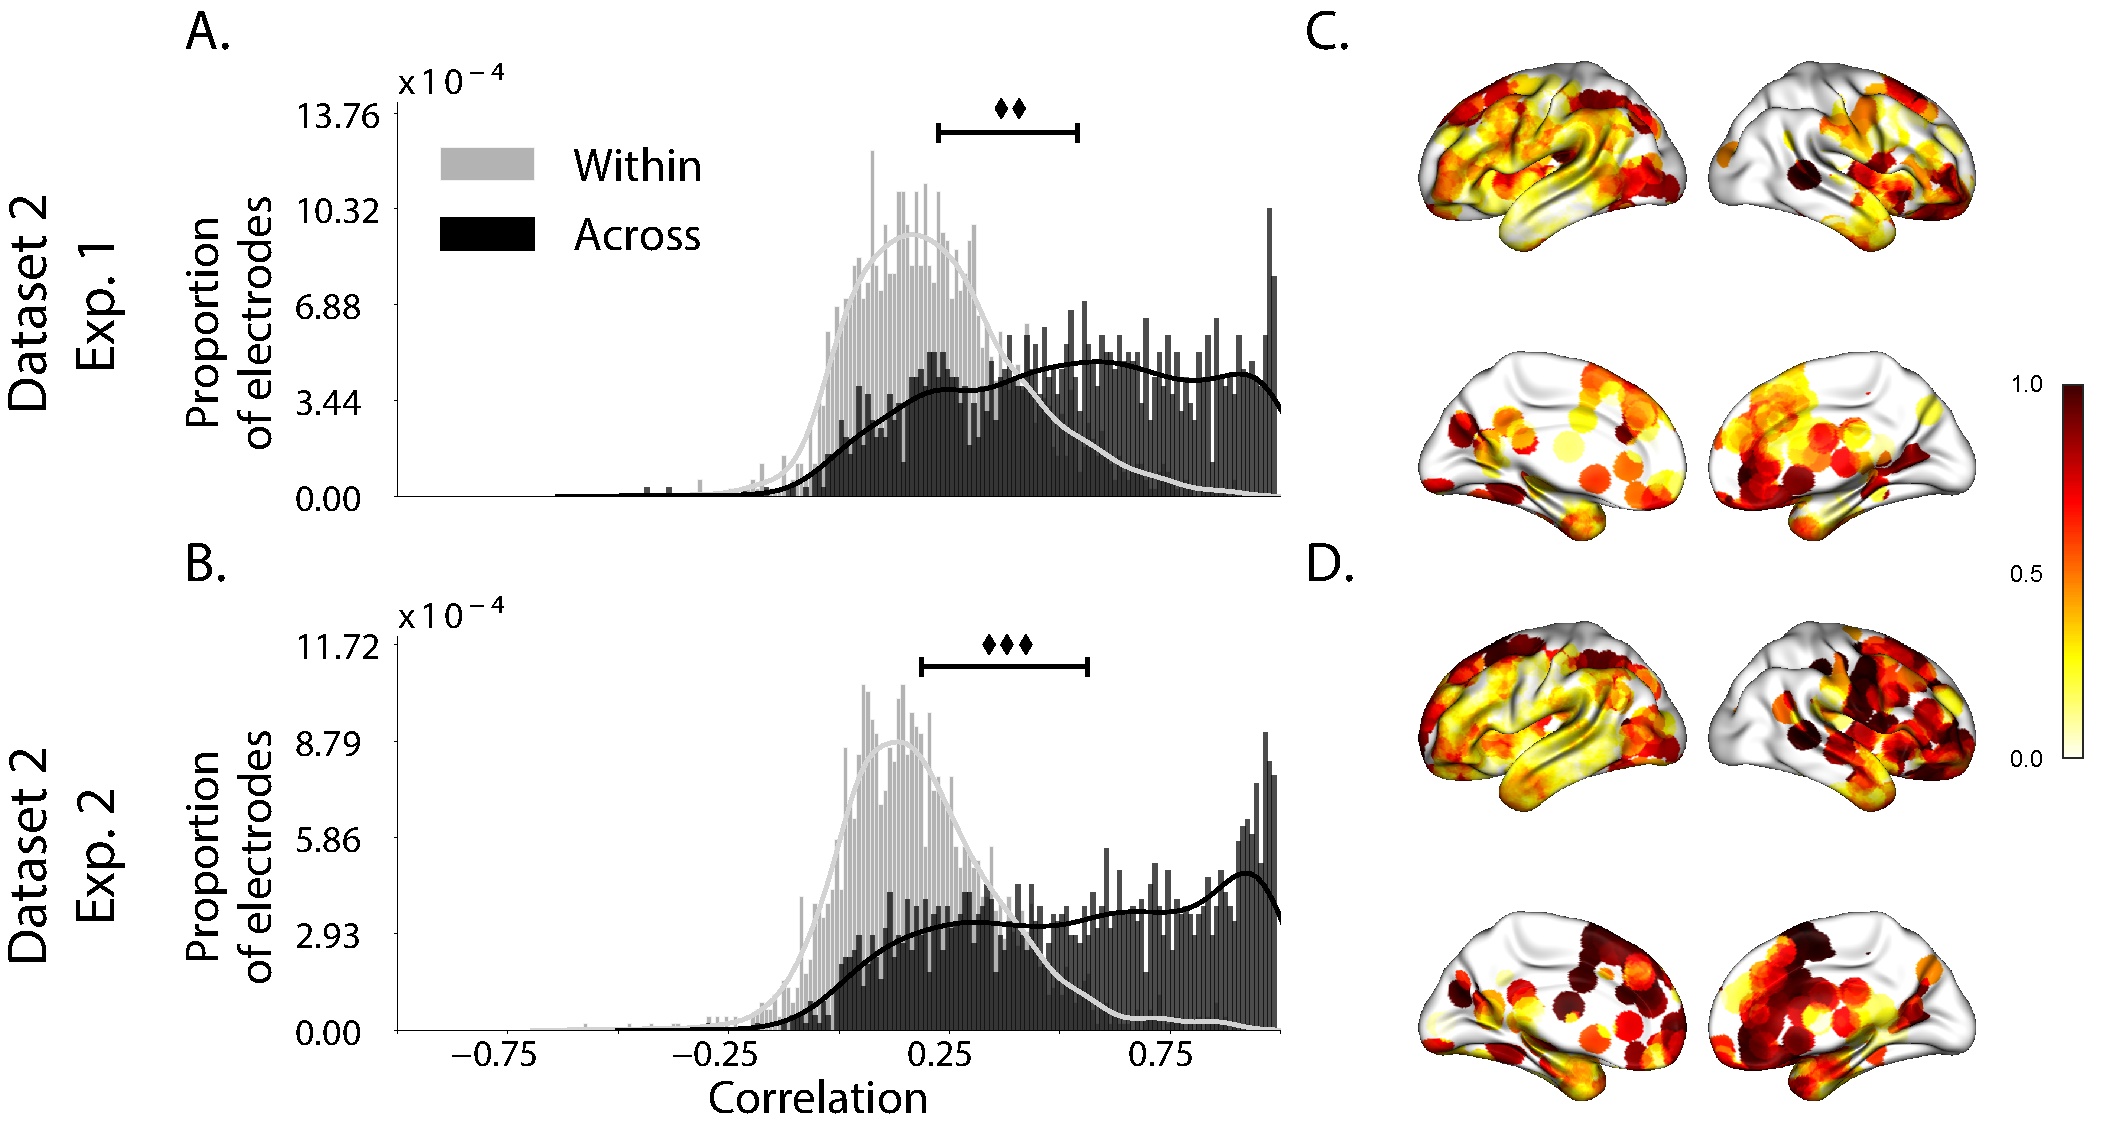
\includegraphics[width=\textwidth]{figs/supplemental_3}
\caption{\textbf{Reconstruction accuracy across all electrodes in Dataset 2.}
This figure is analogous to Figure~\corrmaps~in the main text, but displays data
for Dataset 2 broken down by experiment. \textbf{A. Distributions of
correlations between observed versus reconstructed activity by electrode for
Experiment 1.}  The across-patient distribution (black) reflects reconstruction
accuracy (correlation) using a correlation model learned from all but one
patient's data, and then applied to that held-out patient's data.  The
within-patient distribution (gray) reflects performance using a correlation
model learned from the same patient who contributed the to-be-reconstructed
electrode. \textbf{B. Distributions of correlations for Experiment 2.}  This
panel is in the same format as Panel A, but reflects results obtained from
Experiment 2. \textbf{C.--D. Reconstruction accuracy by location.} The colors
denote the average across-session correlations, using the across-patient
correlation model, between the observed and reconstructed activity at the given
electrode location projected to the cortical surface~\citep{CombEtal19}.  Panel
C displays the map for Experiment 1 and Panel D displays the map for Experiment 2.}
\label{fig:supplemental_3}
\end{figure}


\begin{figure}[p]
\centering
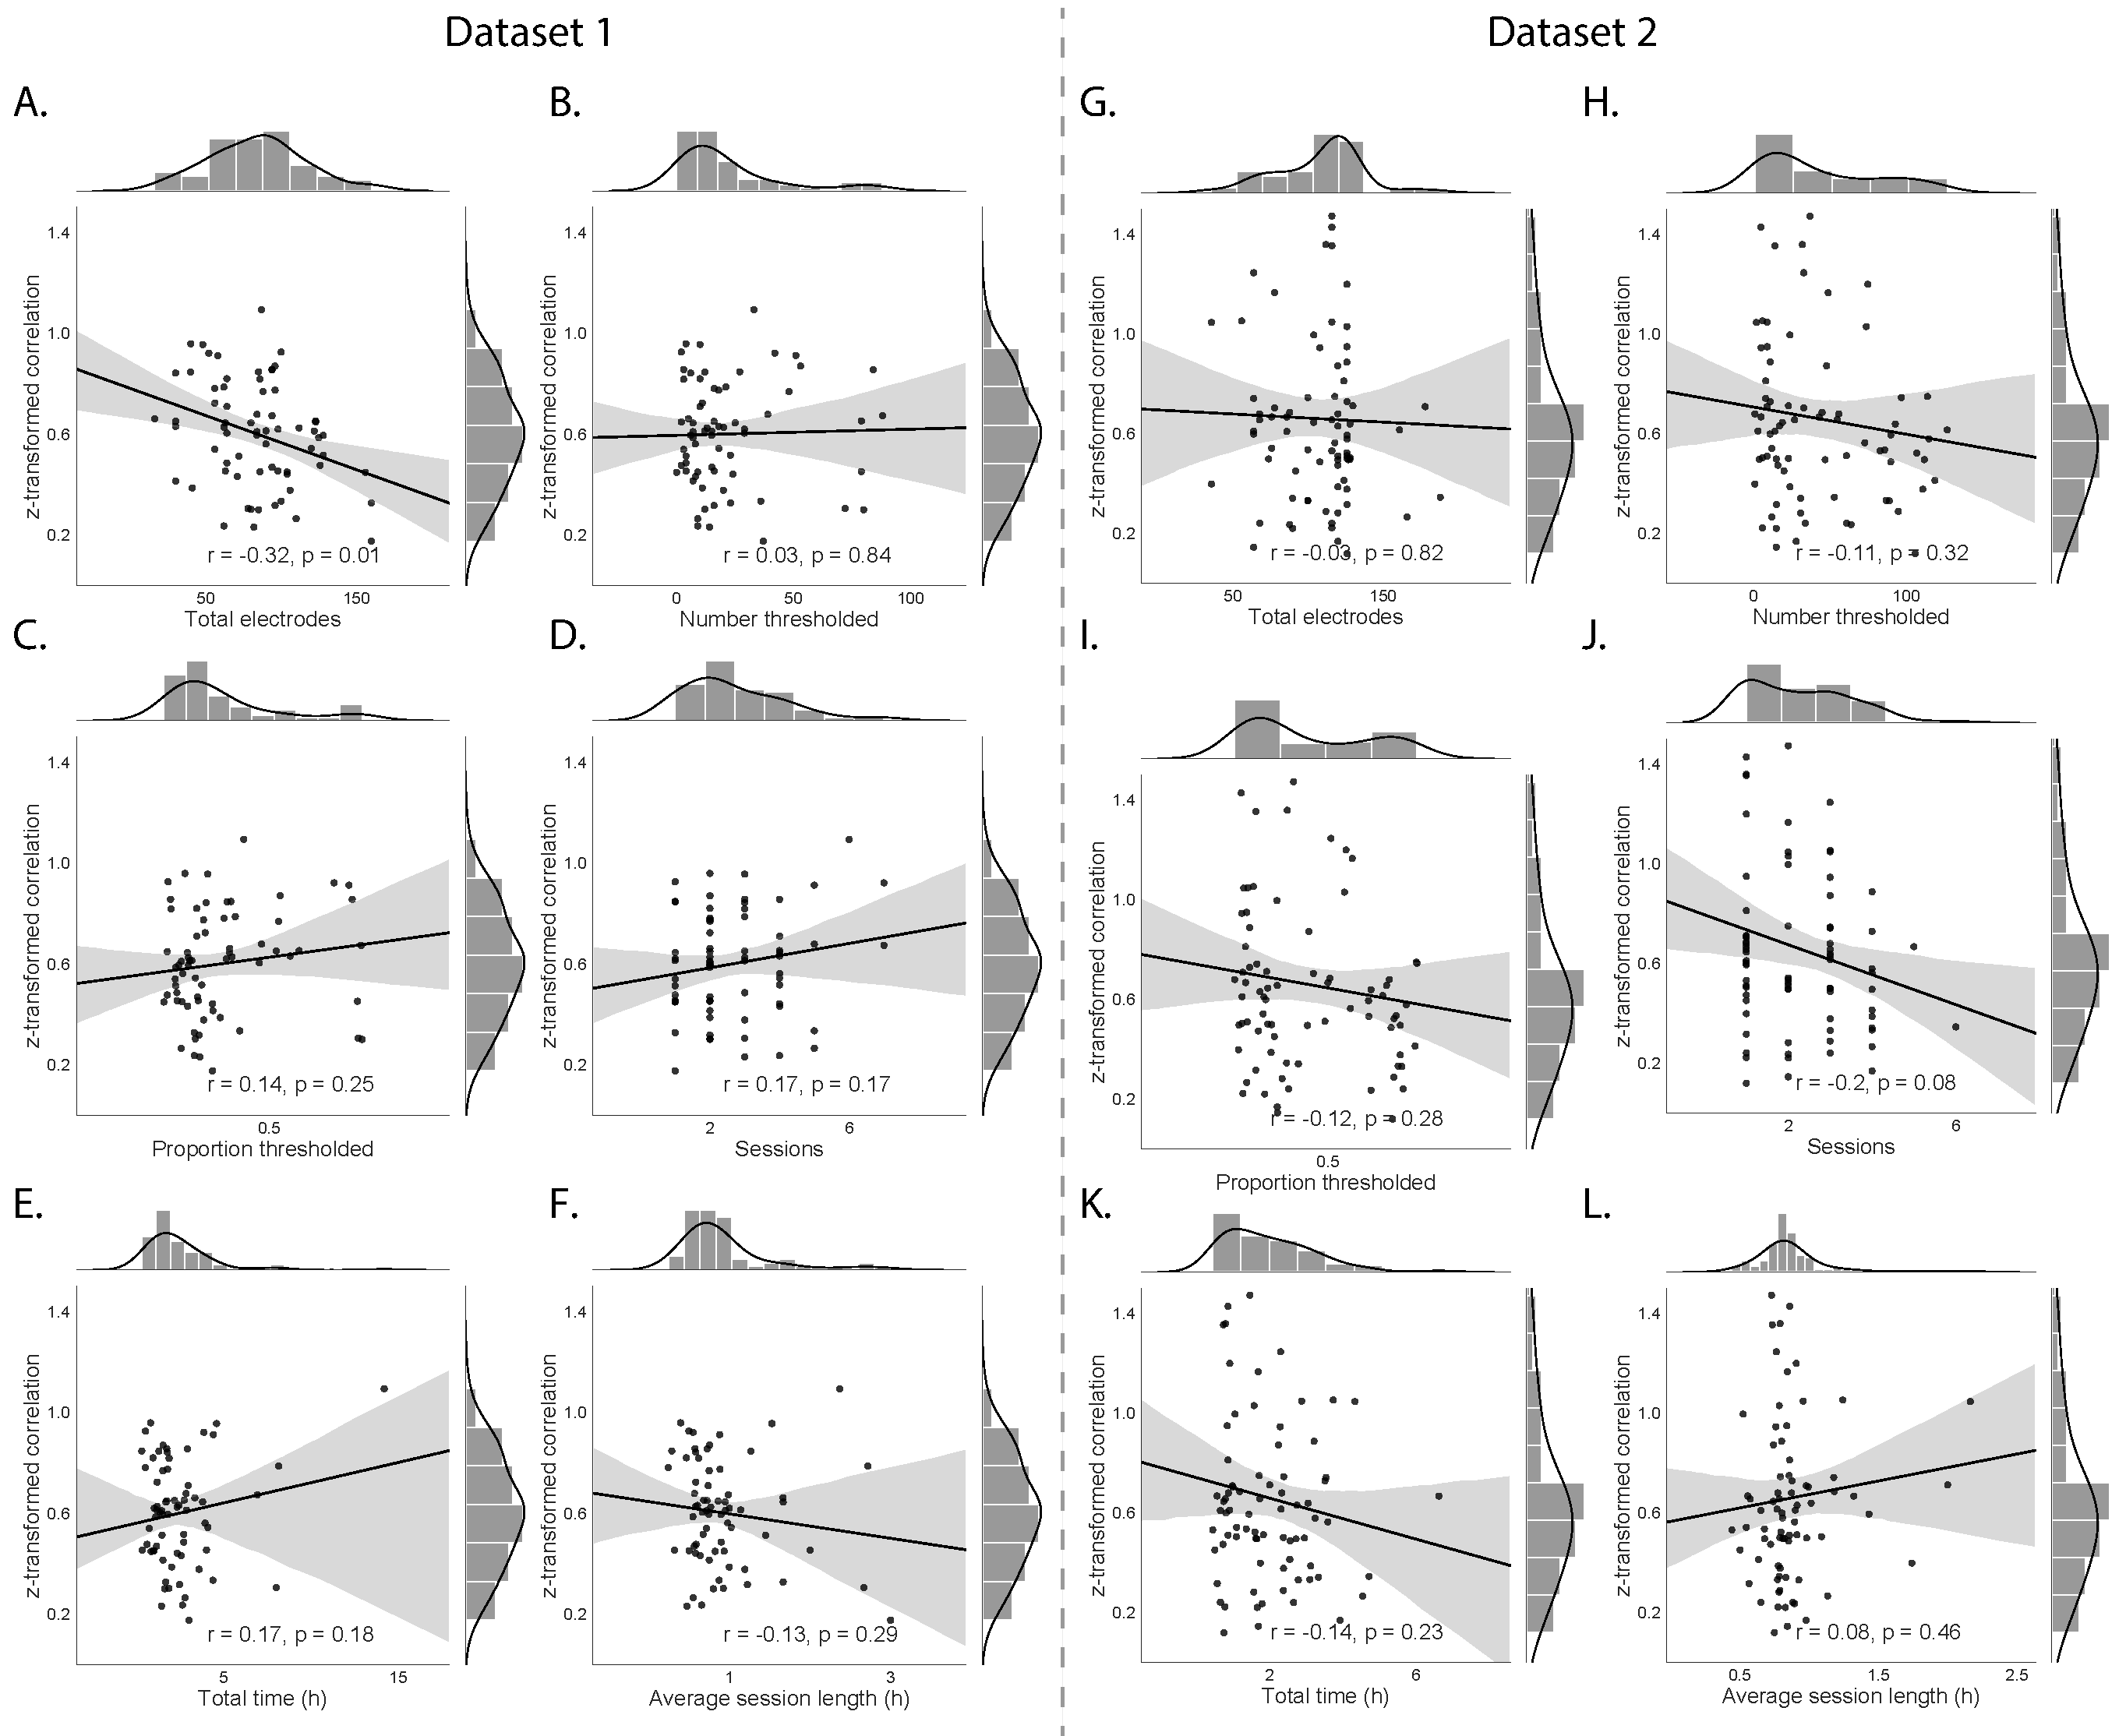
\includegraphics[width=\textwidth]{figs/supplemental_4}
\caption{\textbf{Reconstruction accuracy across all electrodes in two ECoG
datasets for power in each frequency band.} This figure is analogous to
Figure~\freqs~in the main text, but displays the reconstruction accuracies of
the \textit{power} in each frequency band, rather than the bandpass-filtered
voltages, as in Figure~\freqs. \textbf{A. Distributions of correlations between
observed versus reconstructed power by electrode for each frequency band in
Dataset 1.}  Each color denotes a different frequency band. Within each color
group, the darker dots and bar on the left display the distribution (and mean)
across-patient reconstruction accuracies (analogous to the black histograms in
Fig.~\corrmaps).  The lighter dots and bar on the right display the distribution
(and mean) within-patient reconstruction accuracies (analogous to the gray
histograms in Fig.~\corrmaps). Each dot indicates the reconstruction accuracy
for one electrode in the dataset. \textbf{B.~Statistical summary of
across-patient reconstruction accuracy by electrode for each frequency band in
Dataset 1.} In the upper triangles of each map, warmer colors (positive
$t$-values) indicate that the reconstruction accuracy for the frequency band in
the given row was greater (via a two-tailed paired-sample $t$-test) than for the
frequency band in the given column. Cooler colors (negative $t$-values) indicate
that reconstruction accuracy for the frequency band in the given row was lower
than for the frequency band in the given column. The lower triangles of each map
denote the corresponding $p$-values for the $t$-tests. The diagonal entries
display the average reconstruction accuracy within each frequency band.
\textbf{C.~Statistical summary of within-patient reconstruction accuracy by
electrode for each frequency band in Dataset 1.} This panel displays the
within-patient statistical summary, in the same format as Panel B.
\textbf{D.~Distributions of correlations between observed versus reconstructed
activity by electrode, for each frequency band in Dataset 2.} This panel
displays reconstruction accuracy distributions for each frequency band for
Dataset 2. \textbf{E.--F.~Statistical summaries of across-patient and
within-patient reconstruction accuracy by electrode for each frequency band in
Dataset 2.} These panels are in the same as Panels B and C, but display results
from Dataset 2.}
\label{fig:supplemental_4}
\end{figure}


\begin{figure}[p]
\centering 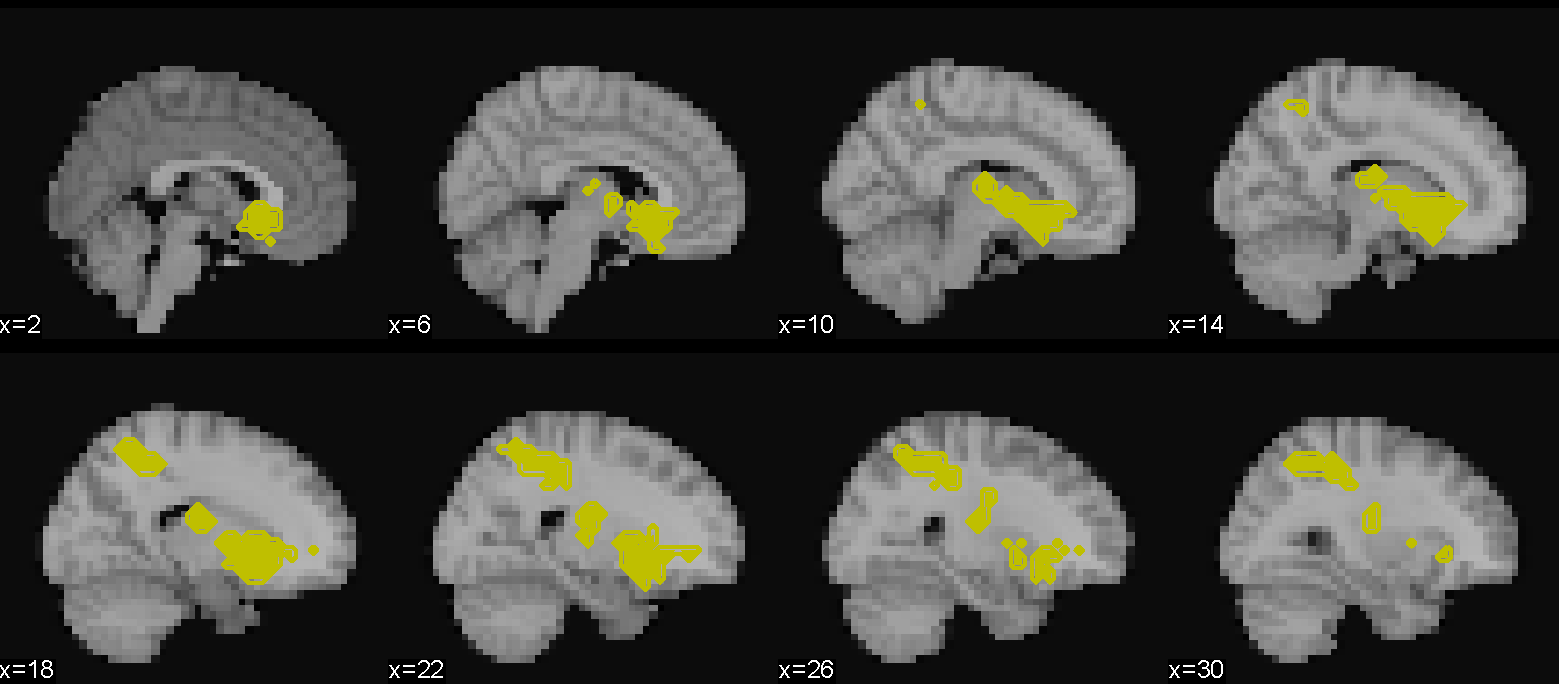
\includegraphics[width=\textwidth]{figs/supplemental_5}
\caption{\textbf{Most informative recording locations by frequency band.} This
figure is analogous to Figure~\infomapfreqs~in the main text, but displays the
brain regions that were most informative about the \textit{power} in each
frequency band (whereas Fig.~\infomapfreqs~displays the regions that were most
informative about the bandpass-filtered voltages within each band).
\textbf{A.~Intersections between information score maps by frequency band.} The
regions indicated in each row depict the intersection between the top 10\% most
informative locations across Datasets 1 and 2.  \textbf{B.~Network memberships
of the most informative brain regions.}  The pie charts display the proportions
of voxels in each region that belong to the seven networks identified by
\cite{YeoEtal11}.  The relative sizes of the charts for each frequency band
reflect the average across-subject reconstruction accuracies
(Figs.~\freqs A, D).  The voxels in Panel A are colored according to
the same network memberships.  \textbf{C.~Neurosynth terms associated with the
most informative brain regions, by frequency band.}  The lists in each row
display the top five neurosynth terms~\citep{RubiEtal17} decoded for each
region.  \textbf{D.~Network parcellation map and legend.}  The parcellation
defined by \cite{YeoEtal11} is displayed on the inflated brain maps.  The colors
and network labels serve as a legend for Panels A and B. \textbf{E.~Combined map
of the most informative brain regions.}  The map displays the union of the most
informative maps in Panel A, colored by frequency band.  The labels also serve
as a legend for Panel C.}
\label{fig:supplemental_5}
\end{figure}

\begin{figure}[p]
\centering 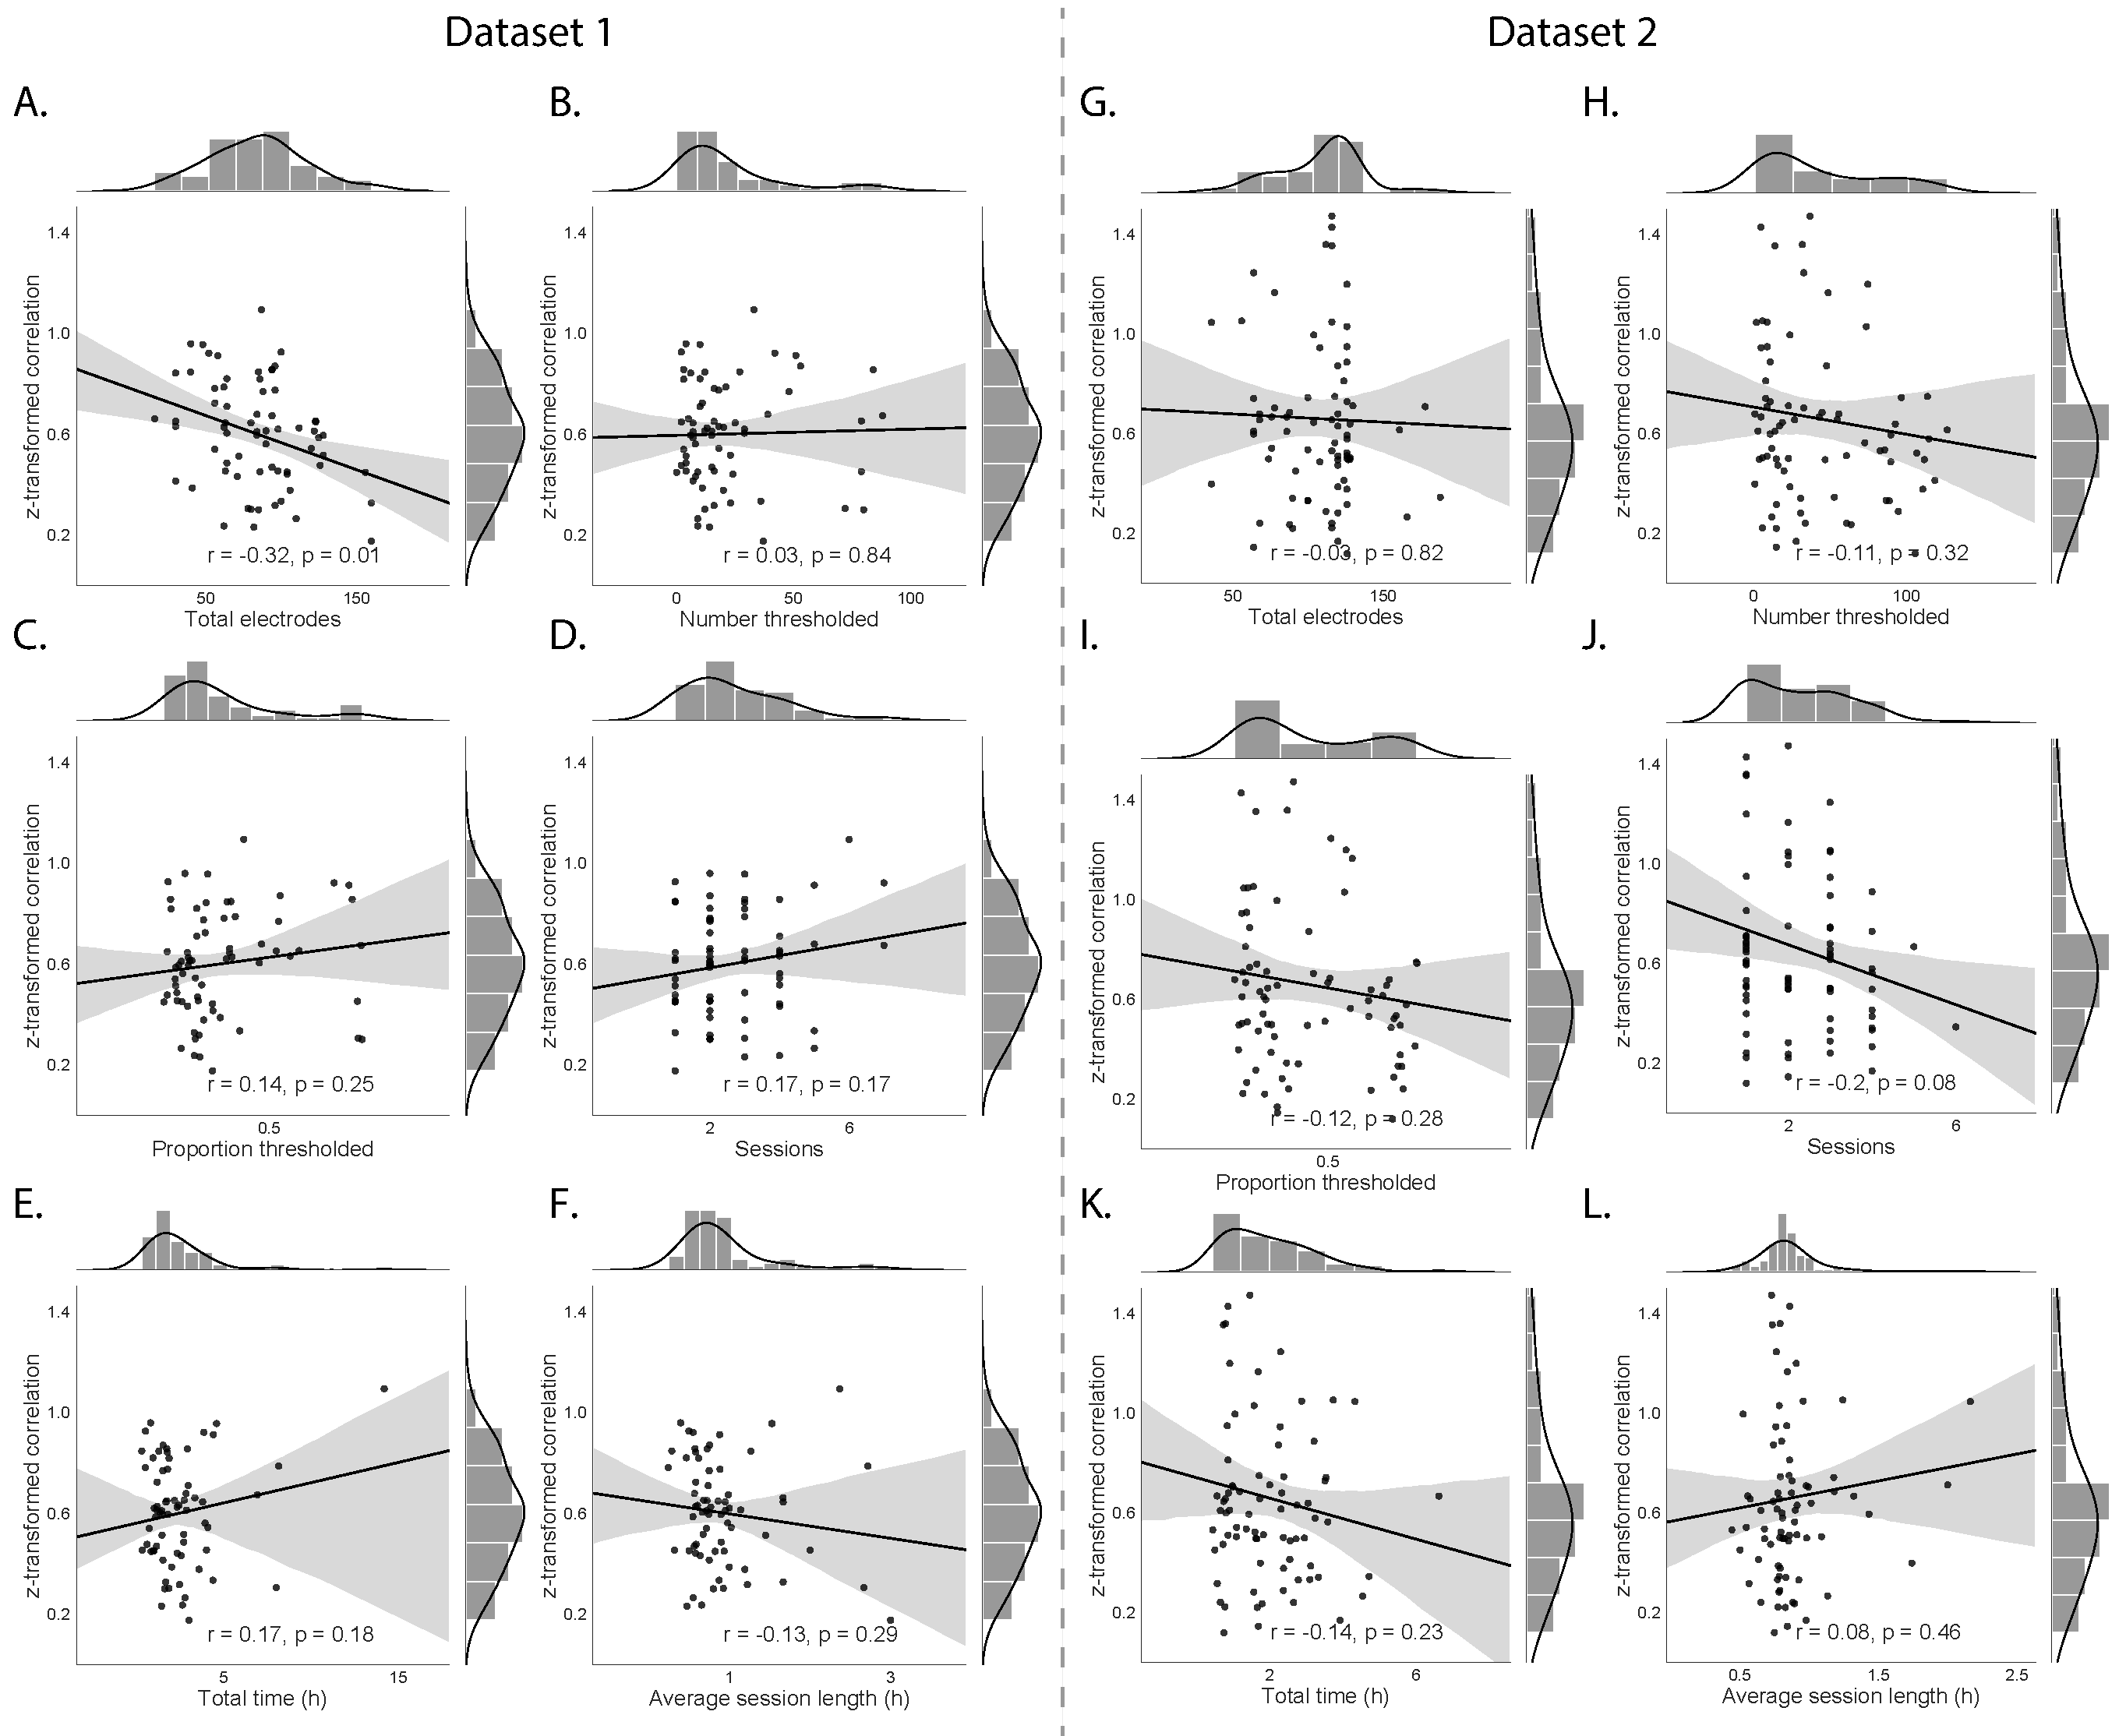
\includegraphics[width=\textwidth]{figs/supplemental_6}
\caption{\textbf{Reconstruction accuracy versus within-subject data features for
two ECoG datasets.} The individual dots in each panel  reflect data from one
patient.  The least-squares linear regression lines (with shaded 95\% confidence
intervals) and the correlations reported in each panel are between the data
shown on the $x$- and $y$-axes of the panel.  The $y$-axis in each panel
denotes the average $z$-transformed correlation between the observed and
predicted voltage timeseries at each electrode (across all of the patient's
electrodes). The cross-validated predictions were obtained using the
across-patient model (Fig.~\corrmaps A and B, black histograms).  \textbf{A.--F.
Dataset 1.}  \textbf{A. Total electrodes.}  The $x$-coordinates of each dot
display the total number of electrodes implanted in each patient's brain.
\textbf{B. Number thresholded.}  The $x$-coordinates of each dot display the
number of implanted electrodes that survived the kurtosis-based filtering
procedure (see \textit{Approach}).  \textbf{C. Proportion thresholded.} The
$x$-coordinates of each dot display the \textit{proportion} of each patient's
implanted electrodes (relative to the total number) that survived the
kurtosis-based filtering procedure.  \textbf{D. Sessions.}  The $x$-coordinates of each dot display the
number of distinct recording sessions contributed by each patient.  \textbf{E. Total time.} The $x$-coordinates of each dot display the
total duration (in hours) of each patient's recordings, across all of their recording sessions.  \textbf{F. Average session length.} The $x$-coordinates of each dot display average duration (in hours) of the patient's recording sessions.
  \textbf{G.--L. Features from Dataset 2.}  These panels display analogous information to Panels A--F, but for Dataset 2 patients.}
\label{fig:supplemental_6}
\end{figure}

%JRM STOPPED HERE
\begin{figure}[p]
\centering 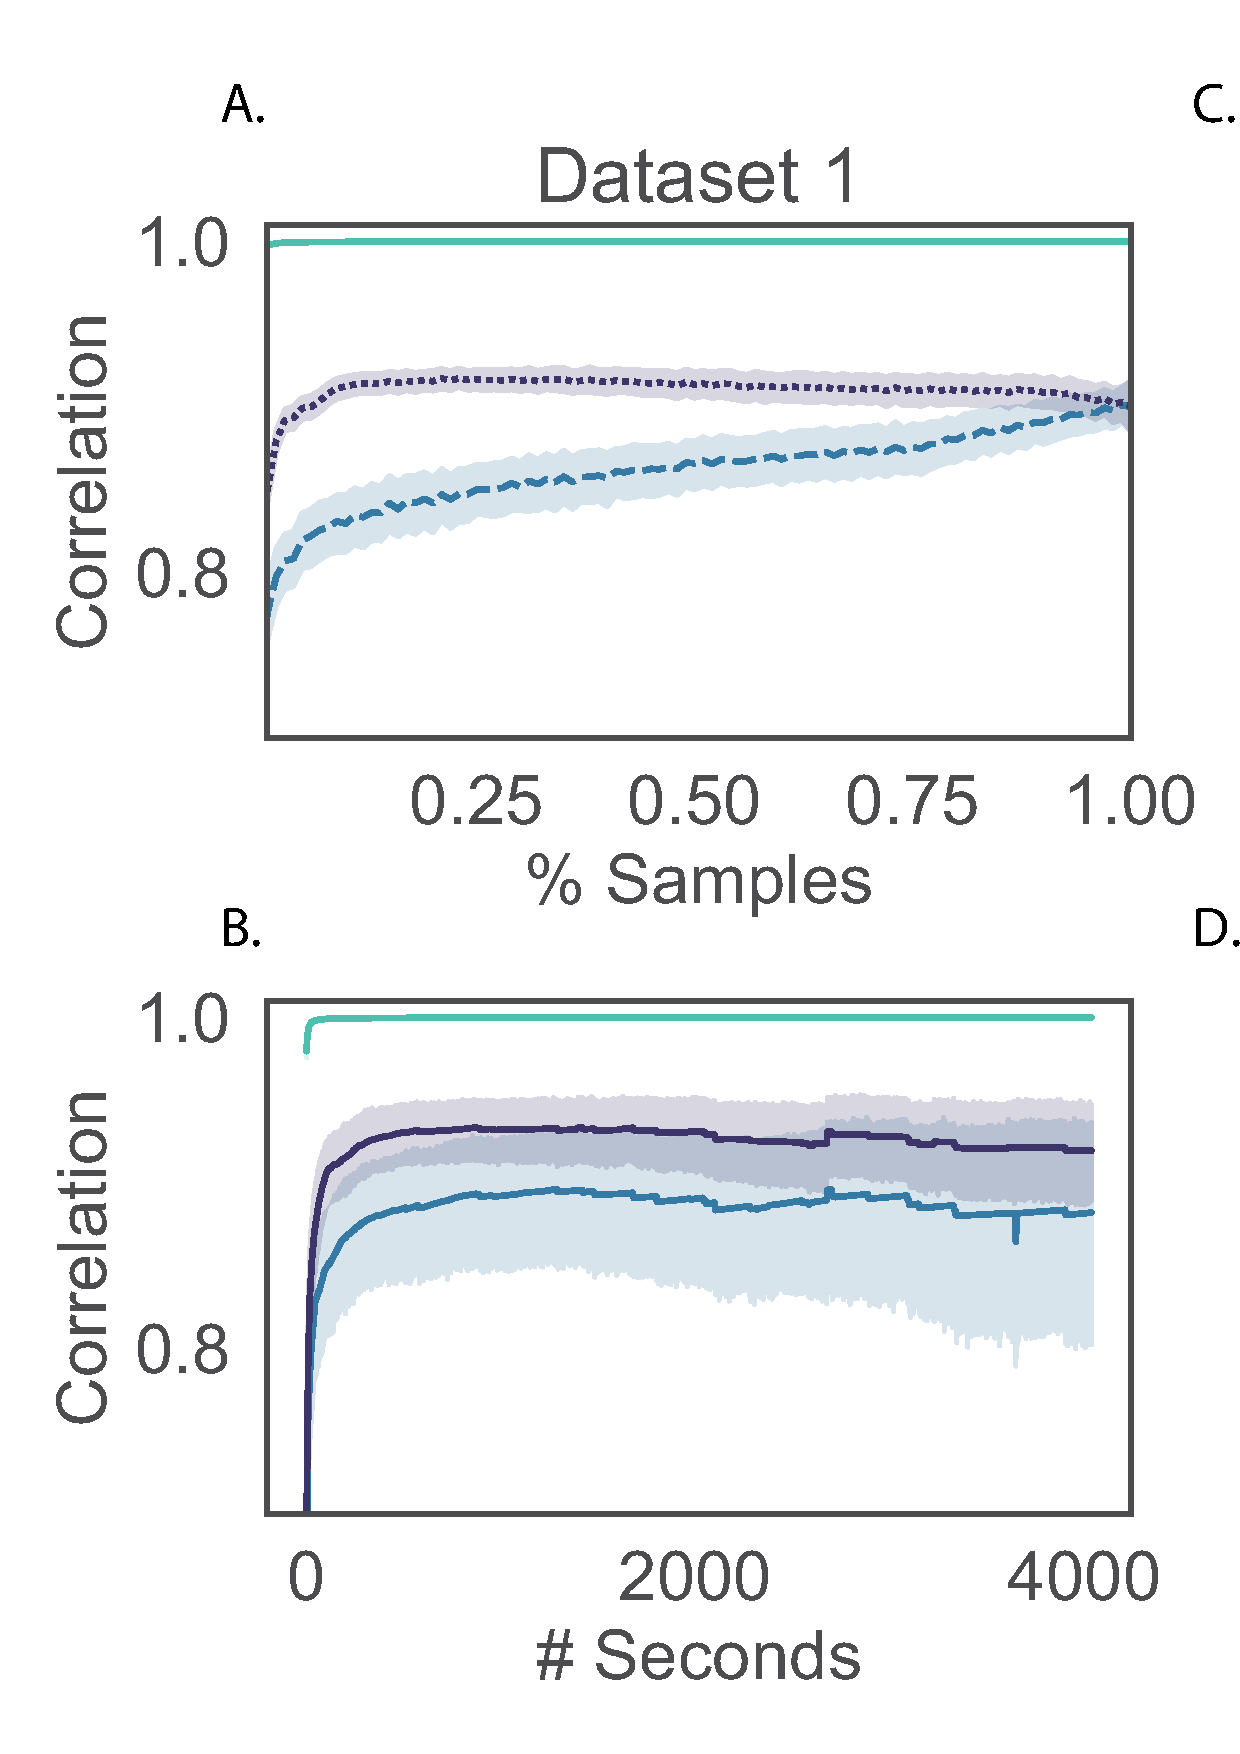
\includegraphics[width=\textwidth]{figs/supplemental_7}
\caption{\textbf{Temporal stability of estimated patient-specific
    correlation matrices.}  For each patient $s$, we computed their
  patient-specific correlation matrix ($C_s$) using two different
  subsets of their recorded data.  We correlated the upper triangles
  of these estimates of $C_s$ to obtain a single correlation for each
  participant, reflecting how stable (in time) the estimates were.  We
  computed this stability measure, for each patient, as a function of
  how much data was used to estimate each $C_s$ (expressed as a
  proportion of the patient's total dataset, as in Panels \textbf{A}
  and \textbf{C}; or as the total duration of the patient's
  recordings, as in Panels \textbf{B} and \textbf{D}).  We also varied
  how the timepoints that went into each estimate were
  related. Specifically, we first concatenated the data from each
  patient's recording sessions to construct a single data timeseries
  (ignoring session boundaries) for each patient.  We then constructed
  two estimates of $C_s$ by drawing each patient's data from two
  equally sized sets of $t$ timepoints chosen from their multi-session
  data matrix.  These timepoints were drawn either at \textit{random}
  without replacement (teal lines); from equally sized timespans at
  the start and end of the multi-session data matrix (\textit{apart},
  blue lines); or from two equally sized timespans just prior to and
  just after the data midpoint (\textit{close}, purple lines).  For
  the random condition of this analysis, as we increased $t$, we
  ensured that all of the timepoints included in the analysis for
  smaller values of $t$ were also included in the analyses for larger
  values of $t$.  For example, the randomly drawn timepoints for
  $t = 2000$ included the same timepoints drawn for $t = 1000$, plus
  an additional 1000 new timepoints.  Panels A and B display the
  resulting correlations for Dataset 1, and panels C and D display the
  correlations for Dataset 2.  Error ribbons in all panels denote 95\%
  confidence intervals (computed across patients).}
\label{fig:supplemental_7}
\end{figure}

\begin{figure}[p]
\centering 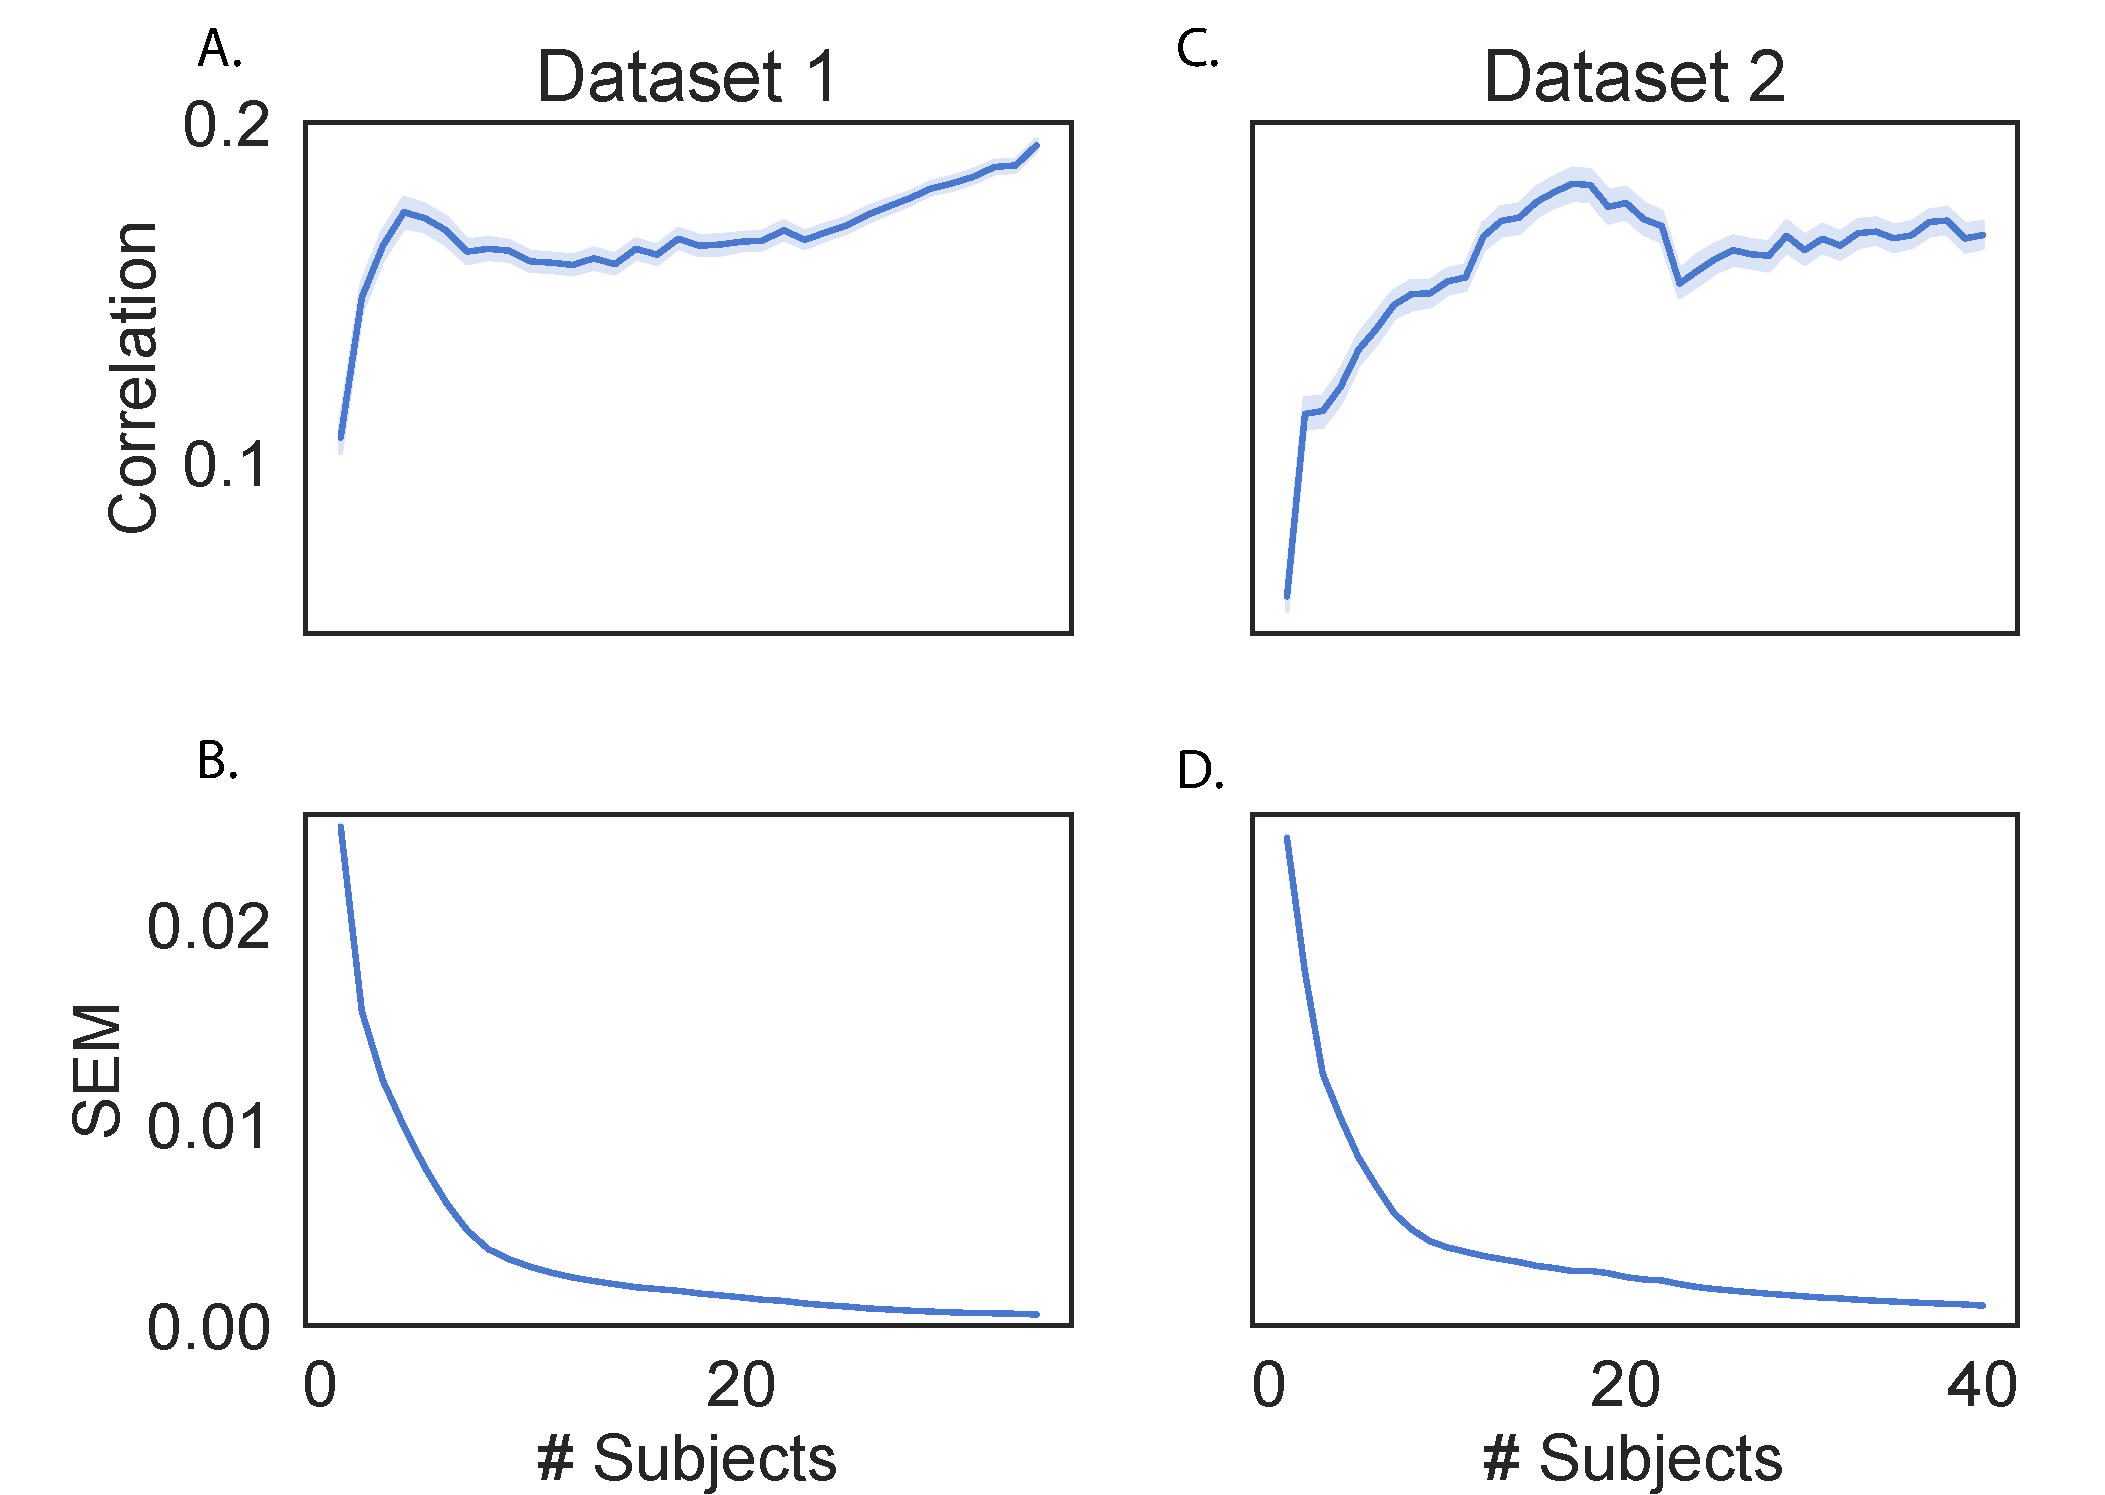
\includegraphics[width=\textwidth]{figs/supplemental_8}
\caption{\textbf{Stability of full-brain correlation matrices across
    patients.}  We estimated full-brain correlation matrices
  ($\hat{K}$) using different subsets of patients from each
  dataset. We explored how stable these estimates were as a function
  of how many patients were used to compute $\hat{K}$. For each sample
  size $n$ (number of patients), we drew two non-overlapping sets of
  $n$ patients (without replacement) from the full set of patients in
  each dataset. We then estimated $\hat{K}$ using the two sets of $n$
  patients.  We computed the correlation between the upper triangles
  of these matrices as a measure of how similar the matrices were.  We
  repeated this procedure 500 times for each value of $n$ (ranging
  from 1 up to $\frac{1}{2}$ of the total number of patients in the
  given dataset); this yielded a distribution of correlation
  coefficients for each value of $n$.  Panels \textbf{A} and
  \textbf{C} display the mean correlations as a function of $n$ for
  Datasets 1 and 2, respectively.  The error ribbons denote 95\%
  confidence intervals (computed across iterations).  Panels
  \textbf{B} and \textbf{D} display the standard error of the mean
  (SEM) of these distributions of correlations as a function of $n$,
  for Datasets 1 and 2, respectively.  The error ribbons denote
  bootstrap-derived 95\% confidence intervals.}
\label{fig:supplemental_8}
\end{figure}

\clearpage
\newpage
\renewcommand{\refname}{Supplemental references}
\renewcommand{\bibnumfmt}[1]{[S#1]}
\renewcommand{\citenumfont}[1]{S#1}
\bibliography{CDL-bibliography/memlab}
\bibliographystyle{CSE}
% \newpage

% \bibliography{memlab}


\end{document}
